% !TeX root = ../main/main.tex
\documentclass[../main/main.tex]{subfiles}

\begin{document}
\espacio

  En este capítulo se muestra el panorama general del problema que se analizará y la importancia teórica y práctica del resultado del análisis.

  \section{Aspectos generales}

  La computación en la nube ha cambiado el paradigma con el que se brindan la mayoría de los servicios web en la actualidad. Pero este cambio de paradigma incluye también algunos problemas, entre ellos, la necesidad de personal especializado en la administración de ambientes de virtualización. Sin embargo, es muy difícil encontrar personas especializadas tanto en el ambiente de infraestructura como en el de seguridad informática. Por lo cual las empresas e instituciones públicas deben contenmplar ahora la contratación de personal de infraestructura y de seguridad conformando un grupo multidisciplinario, con lo que los costos de manteminiento de los sistemas informáticos se incrementa.

  El adelanto en la tecnología llegó a tal punto en que el paradigma de administración de servidores de la decada de los 90 volvió a resurgir pero en ``centros de datos virtualizados''. Éste término se popularizó a finales del año 2004, cuando Amazon lanzó su servicio AWS\footnote{Amazon Web Services}

  La computación en la nube y los centros de datos virtualizados son dos conceptos diferentes. El primero hace referencia al procesamiento de datos en servidores remotos, mientras que el segundo hace referencia a la administración de computadoras y redes virtualizadas, administradas de manera remota.

  En este análisis se utiliza un concepto de virtualización todavía más específico pero que forma parte de los centros de datos virtualizados, la virtualización de aplicaciones mediante contenedores.

  \begin{figure}[ht]
    \centering
    \caption{Administración de servidor AWS con entorno de virtualización Docker}
    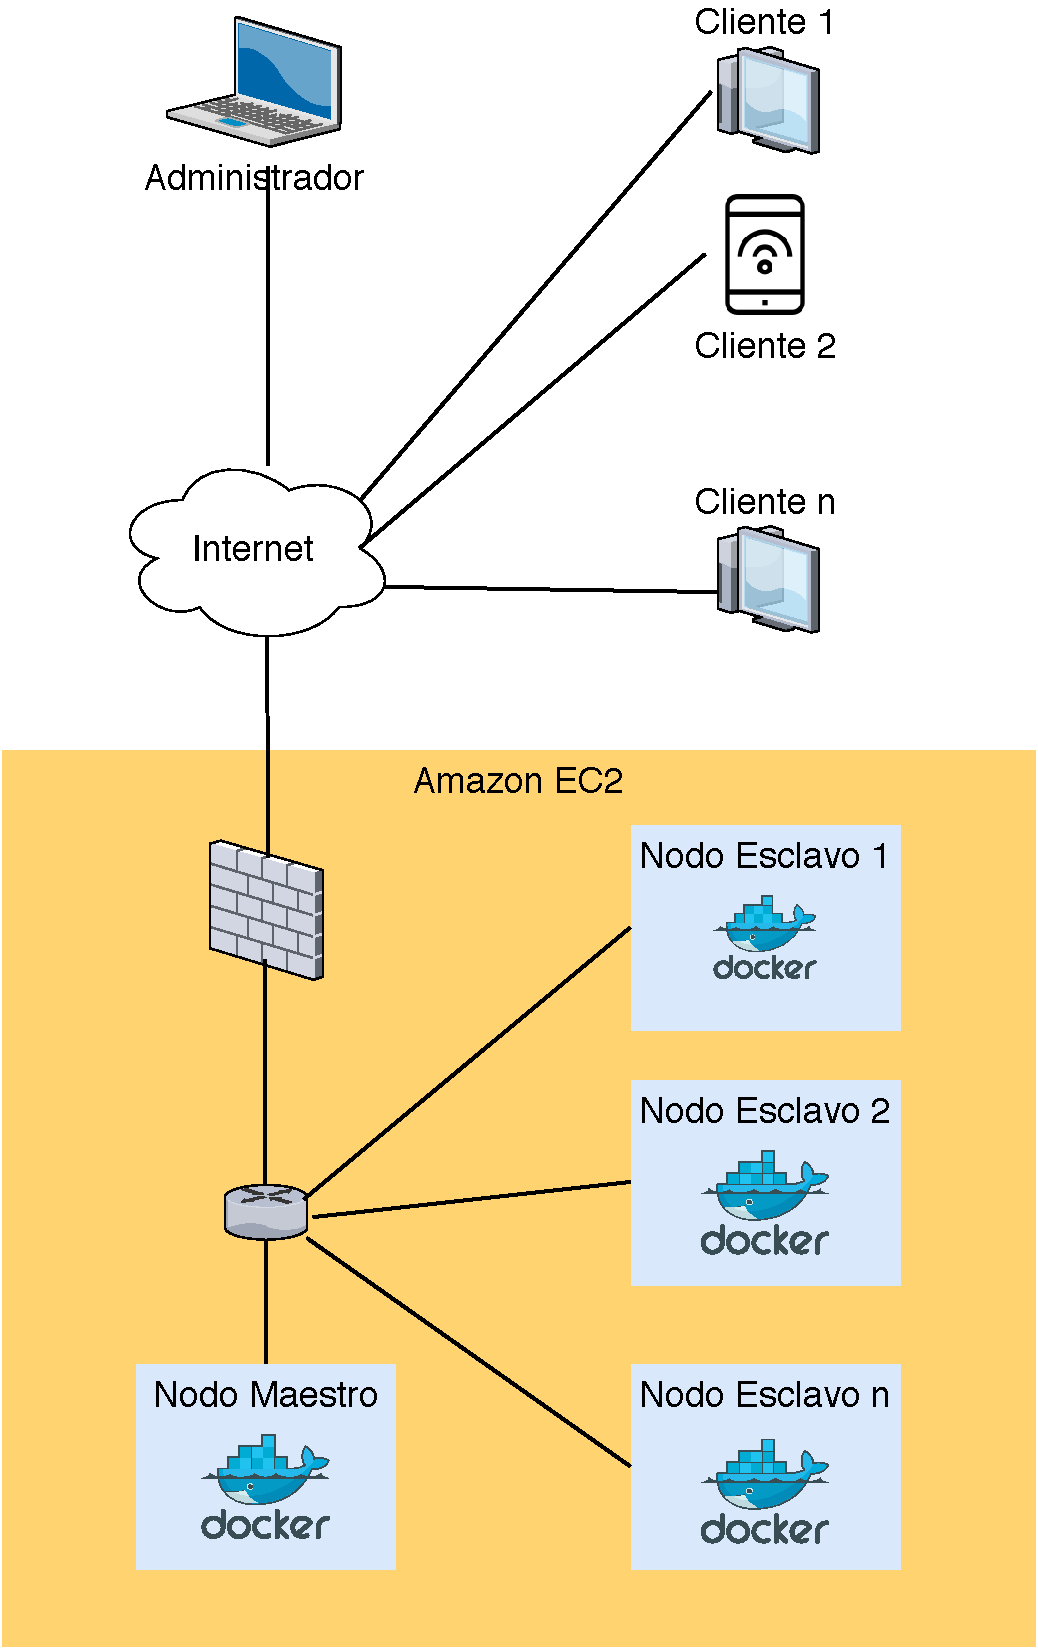
\includegraphics[width=10cm, keepaspectratio]{\main/introduccion/diagrama_aws.pdf}
    \caption*{\textbf{Fuente:} Elaboración propia}
  \end{figure}

  Sin embargo, el campo de la seguridad informática, aún dando sus primeros pasos en Bolivia, es muy importante y no se debe tomar a la ligera porque la tecnología avanza al mismo ritmo para las entidades privadas, públicas, la población y como no podría se de otra manera, para los delincuentes. Es en este sentido que los servidores deben ser protegidos contra una gran cantidad de tipos de ataques, entre uno de ellos está la inyección de código malicioso en las aplicaciones desplegadas, así como en las herramientas utilizadas para el despliegue.

  \section{Importancia teórica y práctica}

  Los entornos de virtualización completa como Hyper-V, VMWare vSphere o KVM son llamados de esta manera ya que se aislan del sistema operativo anfitrión, este tipo de virtualización por lo general requiere de equipos con características especiales para su funcionamiento.

  Los entornos de virtualización basada en contenedores, también conocida como virtualización ligera, son simplemente un conjunto de directorios que contiene librerías y recursos para brindar un servicio específico, este tipo de virtualización genera pseudo máquinas virtuales ligeras y portables que comparten el kernel del sistema operativo anfitrión.

  \begin{figure}[ht]
    \centering
    \caption{Capas de virtualización dentro de un servidor físico}
    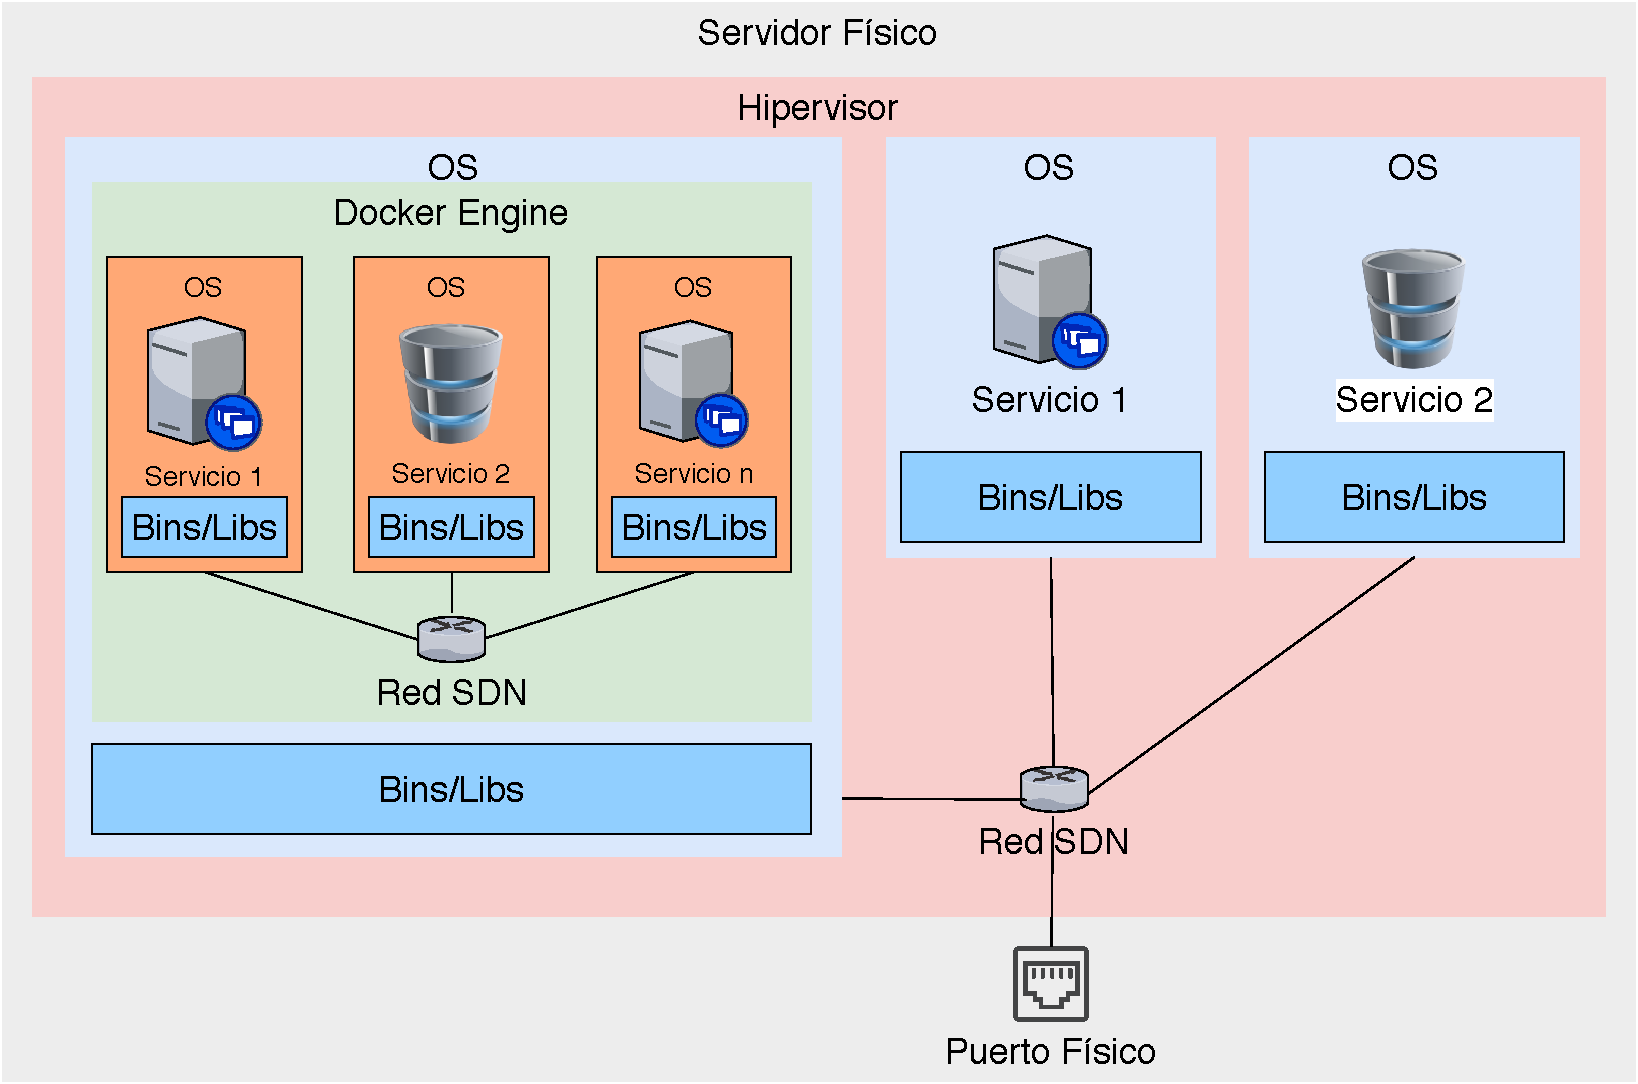
\includegraphics[width=15cm, keepaspectratio]{\main/introduccion/baremetal_kvm_docker.pdf}
    \caption*{\textbf{Fuente:} Elaboración propia}
    \label{fig:baremetal_kvm_docker}
  \end{figure}

  Comúnmente un servidor físico es dividido en máquinas virtuales mediante un hipervisor de virtualización completa y dentro de cada máquinas virtual se despliegan aplicaciones mediante contenedores administrados por un gestor de virtualización ligera como Docker o LXC, como se muestra en la Figura \ref{fig:baremetal_kvm_docker}. De esta manera se generan capas aisladas que mejoran la seguridad, el despliegue de aplicaciones en diferentes entornos y la administración de los servicios.

  Estudiando la distribución de aplicaciones basada en esta forma de administración, la empresa de hardware para seguridad informática  Palo Alto Networks, Inc. reconocida mundialmente, identificó que el gusano Graboid fue insertado en una cantidad considerable de imágenes que sirven de plantilla para muchas aplicaciones distruidas por DockerHub, el servidor oficial de imágenes para Docker.

  La importancia teórica recae en el análisis e identifición del método de infección de este gusano

  Por otra parte, la importancia práctica diverge en dos puntos, el primero es el método de reconocimiento de la infección en contenedores desplegados, acción que nos lleva a subsanar el segundo punto que es la infección en los clientes de dichos contenedores. Por tanto, la importancia del reconocimiento de esta infección es directamente proporcional al número de clientes que hacen uso del servicio infectado, para de esta manera, poder descartar el mal funcionamiento del hardware en equipos cliente tomando en cuenta el bajo rendimiento inesperado generado por la infección de este gusano.

\end{document}